%==================================================
%% chapter03.tex for NWPU Bachelor Thesis
%% Encoding: UTF-8
%%==================================================

\chapter{实验与结果}
\label{chap:Results}

\section{概述}
\label{sec:sdcomments}
底层模块主要负责单片机与SD卡的通信和数据传输,可以被上层函数调用。
本文件接口具有良好的可移植性,本实验过程中,选用C8051F020芯片作为示例,
该芯片带有硬件SPI模块,可以直接与SD卡相关引脚连接实现SPI通信。
本章主要描述底层模块,即SD卡硬件模块,在具体实验环境中的设计与实现过程,
同时会对SD卡及本实验选用的SPI模式作以说明。
该模块为上层模块预留的API如下所示:
\begin{lstlisting}[language={C}, caption={底层模块API}]
// Prototypes for disk control functions
DRESULT disk_initialize (BYTE *type);           //底层硬件的初始化
DRESULT disk_read (BYTE* buff, DWORD sector);   //读扇区块
DRESULT disk_write (BYTE* buff, DWORD sector);  //写扇区块
DRESULT disk_offset(DWORD sec);
\end{lstlisting}

\section{SD卡概要}
\label{sec:sdinfo}
SD卡(即安全数位卡)是一种被设计用来满足安全、容量以及性能的需求的便携式存储卡,
就其容量而言,有三种SD卡:
\begin{itemize}[noitemsep,topsep=0pt,parsep=0pt,partopsep=0pt]
    \item Standard Capacity SD Memory Card(SDSC),即标准容量安全数位卡,支持的最大容量是2GB($2^{31} bytes$),
        并且兼容所有版本的物理层(Physical Layer)规格。
    \item High Capacity SD Memory Card(SDHC),即大容量安全数位卡,支持的容量从2GB到32GB($2^{35} bytes$),
        其定义在物理层规格版本-2.00(Physical Layer Specification Version 2.00)上。
    \item Extended Capcity SD Memory Card(SDXC),即扩展容量安全数位卡,支持容量从32GB到2TB($2^{41} bytes$)。
\end{itemize}
\noindent SD卡就速度而言,又定义了五个速度等级:
\begin{itemize}[noitemsep,topsep=0pt,parsep=0pt,partopsep=0pt]
    \item Class 0 \quad 此类卡并未特别指定速度性能(包含主要定义在PLSV2.0之前的老式SD卡)
    \item Class 2\quad 不低于2MB/sec\footnote{此处的「MB/sec」指$1000\times1000$「Bytes/sec」}的速度性能
    \item Class 4\quad 不低于4MB/sec的速度性能
    \item Class 6\quad 不低于6MB/sec的速度性能
    \item Class 10\quad 不低于10MB/sec的速度性能(高速模式)
\end{itemize}

\subsection{引脚}
\label{sec:pins}
标准SD卡的规格应为$24mm\times32mm\times2.1mm$,具体引脚图可参见图\ref{fig:sdcpin}。
表\ref{tab:sdcpin}显示了各引脚的详细描述及接口细节。

\begin{figure}[!htb]
    \centering
    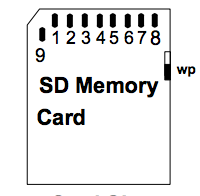
\includegraphics[width=5cm]{chap3/sdc.png}
    \\
    \caption{SDC引脚分布} \label{fig:sdcpin}
\end{figure}

\begin{table}[!htb]
    \centering
    \caption{SD卡引脚在SD模式和SPI模式下的定义}\label{tab:sdcpin}
\begin{threeparttable}
    \begin{tabular}{rccp{2cm}ccp{2cm}}
    \toprule
     & \multicolumn{3}{c}{SD模式} & \multicolumn{3}{c}{SPI模式} \\
    \cmidrule(r){2-4} \cmidrule(r){5-7}
    引脚号& 名称 & 类型\tnote{1}
    & \makecell[c]{描述}& 名称 & 类型\tnote{1} & \makecell[c]{描述}\\ \midrule
    1 & CD/DAT3\tnote{2} & I/O/PP\tnote{3} & 卡检测及数据线「3」  & CS & I\tnote{3} & 片选(低电平使能) \\ \midrule
    2 & CMD & I/O/PP & 命令与应答 & DI & I & 数据输入\\ \midrule
    3 & VSS1 & S & 接地 & VSS & S & 接地 \\ \midrule
    4 & VDD & S & 电源 & VDD & S & 电源 \\ \midrule
    5 & CLK & I & 时钟 & SCLK & I & 时钟 \\ \midrule
    6 & VSS2 & S & 接地 & VSS2 & S & 接地 \\ \midrule
    7 & DAT0 & I/O/PP & 数据线「0」& DO & O/PP & 数据输出 \\ \midrule
    8 & DAT1\tnote{4} & I/O/PP & 数据线「1」& RSV\\ \midrule
    9 & DAT2\tnote{5} & I/O/PP & 数据线「2」& RSV\\
    \bottomrule
    \end{tabular}
    \begin{tablenotes}
    \item [1]「S」:电源;「I」:输入; 「O」: 推挽输出;「PP」:推挽输出/输入。
    \item [2] 扩展的DAT线(DAT1-DAT3)在上电后作为输入。在收到「SET\_BUS\_WIDTH」指令后作为数据线。
    \item [3] 上电后该线有一个$50K\Omega$的上拉电阻,该电阻用于两种功能,卡的检测和模式选择。作为模式选择,
        主机(HOST)将其拉高以选择SD模式,将其拉低以选择SPI模式。作为卡的检测,主机通过命令检测该线是否被拉高。
    \item [4] DATA1可以在SDIO模式中被用于中断输出。
    \item [5] DATA2可以在SDIO模式中被用于读等待信号。
    \end{tablenotes}
\end{threeparttable}
\end{table}

\subsection{寄存器}
\label{sec:register}
每一张卡都有一系列的寄存器用来存储SD卡的相关信息,详见表\ref{tab:reg}。
\begin{table}[!htb]
    \centering
    \caption{SD卡寄存器}\label{tab:reg}
\begin{threeparttable}
    \begin{tabular}{ccp{7cm}}
    \toprule
    名称 & 位宽 & 描述 \\ \midrule
    CID & 128 & Card IDentification number,SD卡识别号,用于身份认证的专属号码 \textbf{必需} \\ \midrule
    RCA\tnote{1} & 16 & Relative Card Address,相对卡址,本地系统的卡地址,初始化时又主机批准 \textbf{必需} \\\midrule
    DSR & 16 & Drive Stage Register,驱动平台寄存器,用来配置卡的输出驱动 \textbf{可选} \\ \midrule
    CSD & 128 & Card Specific Data,卡的具体信息,卡的工作环境信息 \textbf{必需} \\ \midrule
    SCR & 64 & SD Configure Register,SD卡配置寄存器,SD卡具体参数容量信息 \textbf{必需} \\ \midrule
    OCR & 32 & Operation Condition Register,操作环境寄存器 \textbf{必需} \\ \midrule
    SSR & 512 & SD Status Register,卡的所有权信息特性 \textbf{必需}\\ \midrule
    CSR & 32 & Card Status Register,卡信息寄存器,存储了SD卡相关信息 \textbf{必需} \\
    \bottomrule
    \end{tabular}
    \begin{tablenotes}
    \item [1] RCA寄存器在SPI模式不可用
    \end{tablenotes}
\end{threeparttable}
\end{table}

\subsection{SPI模式}
\label{sec:spimode}
SPI模式由基于闪存的SD卡提供的一个次级通信协议组成,该模式是SD卡协议(SD Memory Card Protocol)的一个子集,
被设计用来在SPI标准下中通信。
SPI标准原本只定义了物理层的连接,并不是一个完整的数据传输协议。
SD卡的SPI模式使用了SD卡协议的一个子集及相关的命令集,使得SPI模式具有简便轻量化的优点,
代价就是相对于SD模式损失了部分性能。

\textbf{SPI模式并不支持定义在SD模式(Version 2.0之后)的命令和功能。尽管SD卡处于SPI模式,
    它依然可能对这些命令做出回应,但是,主机(HOST)不应该在SPI模式中使用它们。}



\section{SPI总线协议}
\label{sec:spibus}

SD卡的信道都是基于命令和数据比特流,并且都有起始位和结束位,故SPI信道是字节流的。
每一个命令或者数据块都是基于8比特的字节,并且与CS信号对齐(即使说其长度是8个时钟的倍数)。
当片选信号(CS)使能后,SD卡开始为SPI总线始终计数,每个命令或数据块都必须和8个时钟的边界对齐。
类似于SD卡协议,SPI信息也由命令、回应即数据块令牌组成。所有主机与卡的通信都由主机控制,
主机通过将片选信号(CS)拉低来开始每一次SPI总线上的数据传输。当卡在读操作中进行数据检索时遇到问题时,
它会返回一个错误回应(这个错误回应将取代原本的数据块)。并且,
每一个将数据块写入SD卡的写操作都会得到一个带着数据回答令牌的回应。

对于标准容量卡(SDSC),一个数据块最小是一个字节,最大不超过卡的写入块。

对于大容量卡(SDHC和SDXC),数据块的大小被限制为512字节。同时,写保护命令(CMD28、CMD29、CMD30)不被允许。

\subsection{模式选择和初始化}
\label{sec:modeinit}

SD卡上电后处于SD模式,如果在接收复位命令(CMD0)期间片选信号(CS)保持低电平,那么它将进入SPI模式。
如果卡检测到需求为SD模式则不会对复位命令做出响应,否则将切换至SPI模式同时回应SPI模式的R1。
返回SD模式的唯一方法是重新上电。在SPI模式中,所有SD卡协议的机器将不可见,而SD协议下的命令总是可用的。
图\ref{fig:spiflow}显示了SPI模式的初始化序列。

「SEND\_IF\_COND」命令(CMD8)被用来检测SD卡的工作环境。如果该命令在SD卡视为非法,
那么该卡应为老式卡并且不支持CMD8。

「READ\_OCR」命令(CMD58)被设计用来检测SD卡是否满足主机需求的电压范围。

「SD\_SEND\_OP\_COND」命令(ACMD41)被用来开始初始化并且检测卡是否完成初始化。

初始化完成后需要通过CMD58的回应得到SD卡的CCS信息。当SD卡接受CMD8并且完成初始化后CCS有效。CCS=0表示其为标准容量卡,
CCS=1为大容量卡(SDHC或SDXC)。
\begin{figure}[!htbp]
    \centering
    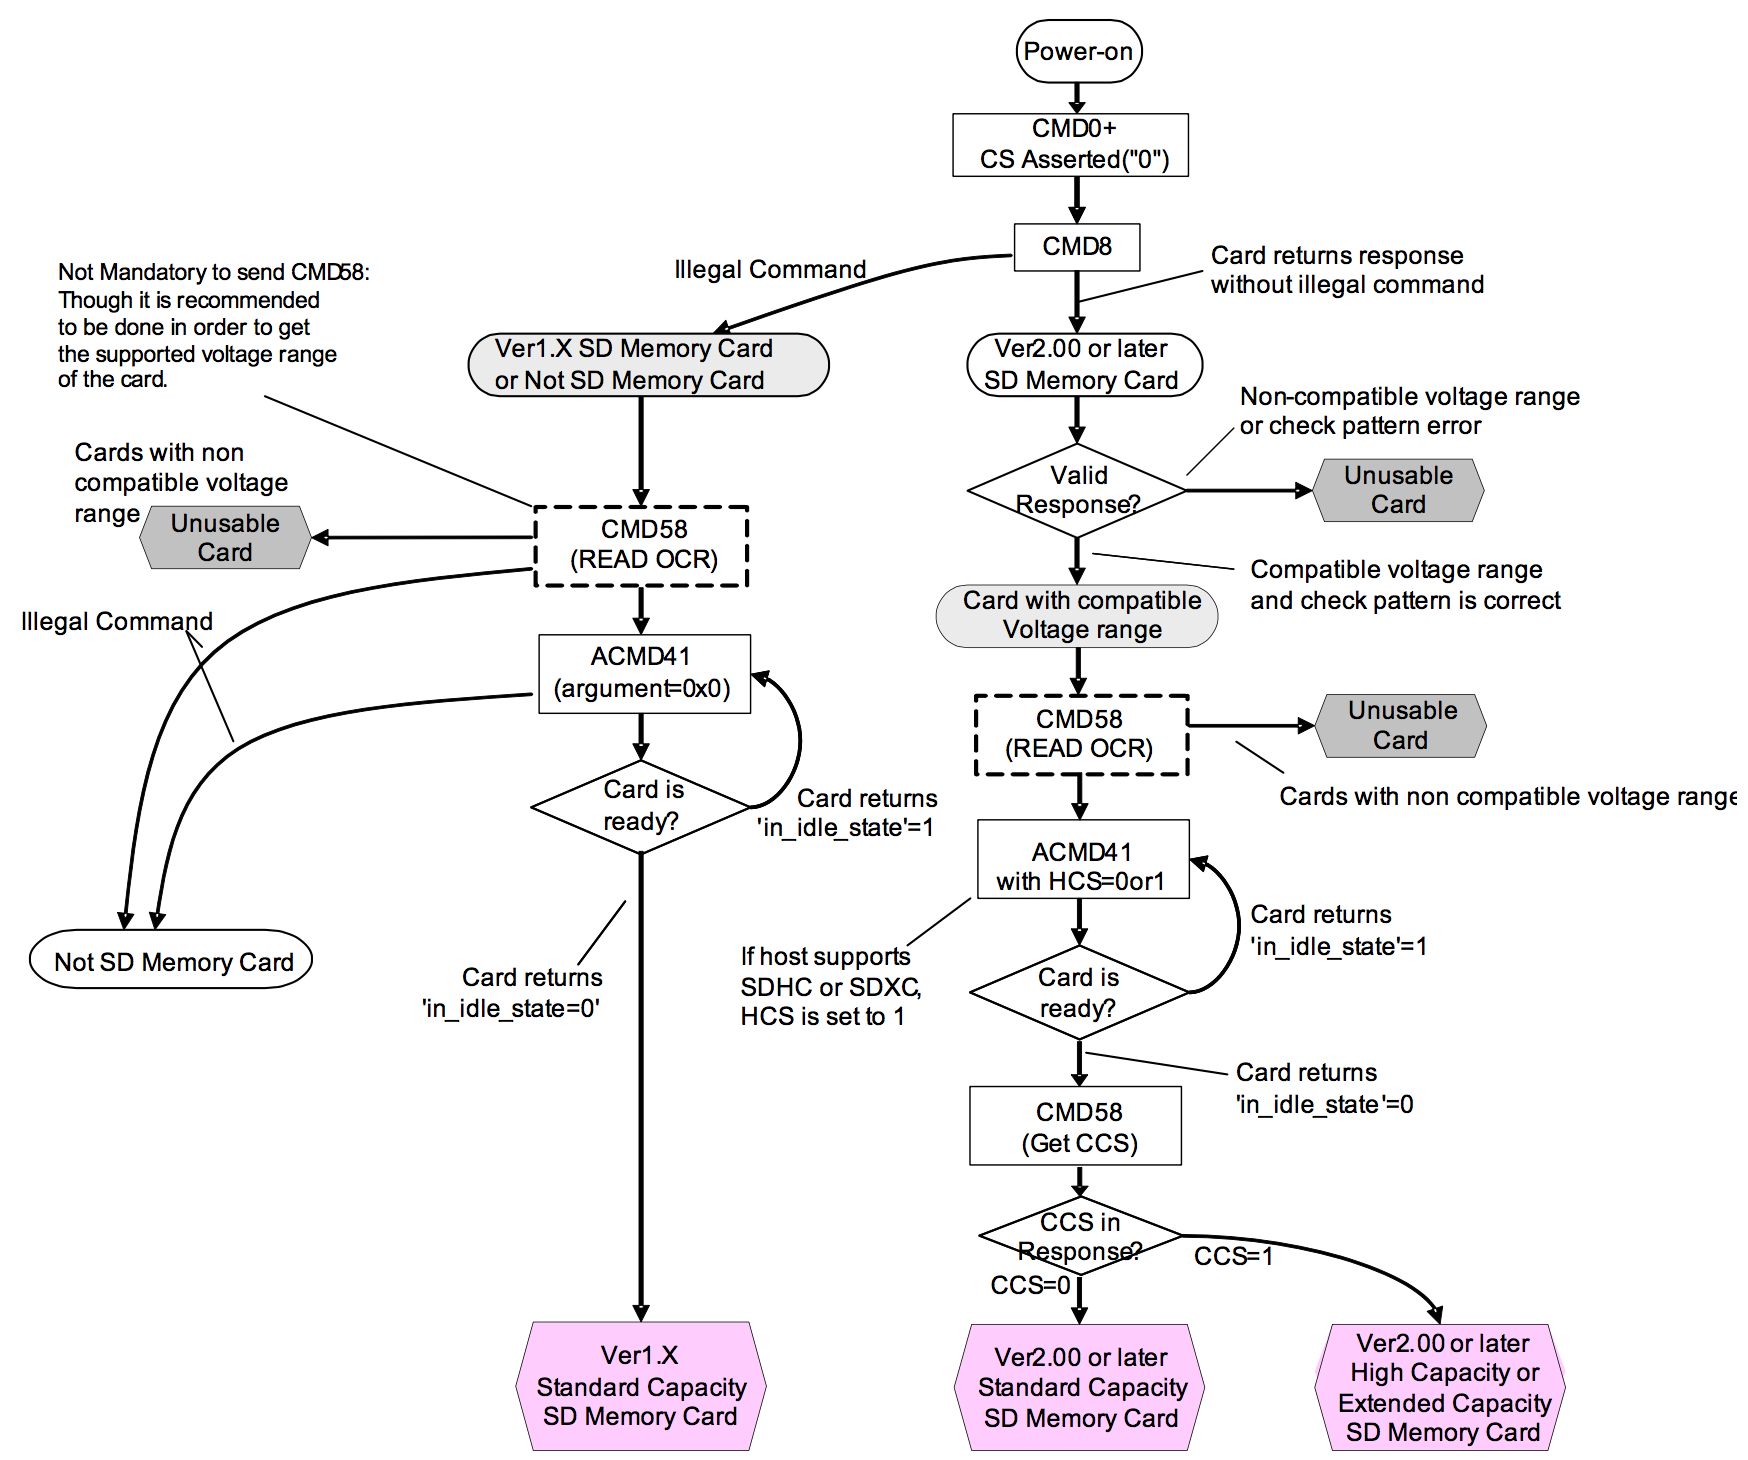
\includegraphics[width=1.0\linewidth]{chap3/spi_flow.png}
    \\
    \caption{SPI模式初始化流程} \label{fig:spiflow}
\end{figure}

初始化流程在图\ref{fig:spiflow}中描述的很详细了,按照顺序发送命令即可。
需要注意的是,初始化时需要采用低速初始化,此时SPI的时钟频率不能超过$400Khz$,本工程使用的是$200Khz$。
初始化结束后可以提升至高速。
这里还有更具体的流程图\ref{fig:specflow},详细描述了每个命令的正确发送时间点及相应的应答格式。
\begin{figure}[!htbp]
    \centering
    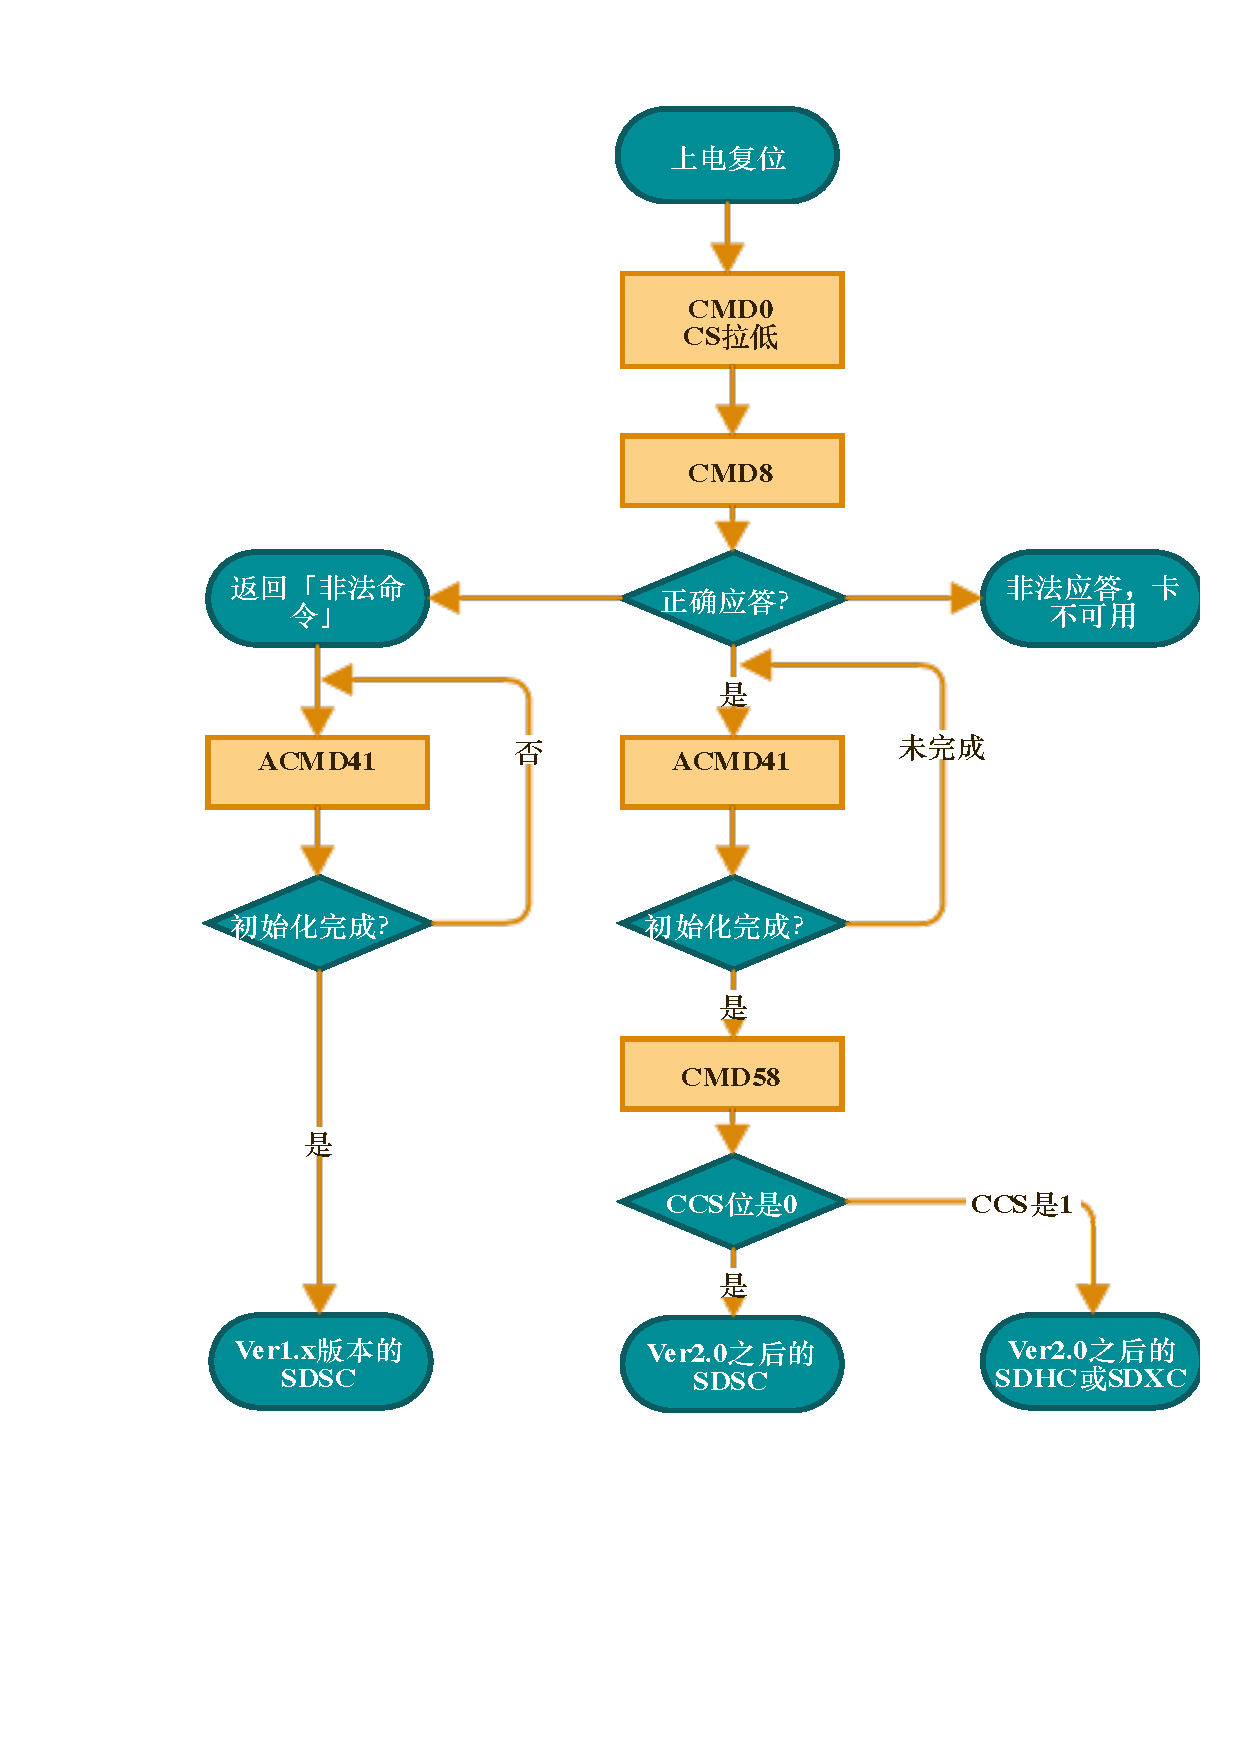
\includegraphics[width=1.0\linewidth]{chap4/specflow.png}
    \\
    \caption{SD卡在SPI模式下的具体初始化流程}\label{fig:specflow}
\end{figure}
发送命令后收到的响应如果不正确,可以循环发送命令直到收到正确应答。对于ACMD41而言,
由于其包含了两个命令(CMD55、ACMD41),故两个命令必需都收到正确应答才算响应正确,否则,两个命令都需要循环发送。
\begin{figure}[!htb]
    \centering
    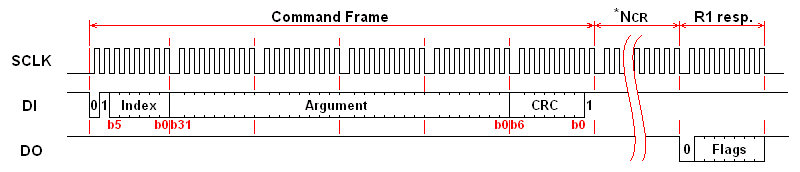
\includegraphics[width=1.0\linewidth]{chap4/cmd.png}
    \\
    \caption{SPI模式下的命令时序}\label{fig:cmd}
\end{figure}
图\ref{fig:cmd}则显示了命令发送时SCK、DI和DO数据线的具体时序。


\subsection{总线数据传输}
\label{sec:datatrans}
每一个SD卡命令在总线上的传输都有CRC校验位的保护,在SPI模式下,同样提供了「CRC ON」的模式来允许系统建立可靠连接。
在「CRC OFF」模式下,命令的CRC校验位会被接收端忽略。SPI接口在初始化时会默认设置为「CRC OFF」模式,然而,
复位命令(RESET,CMD0)是用来切换到SPI模式的,它被接受时SD卡当然尚处于SD模式,所以此时CRC校验位是必需的。
鉴于CMD0命令没有参数,包含CRC校验位在内的所有字节都是常数,故一个合法的复位命令应该为:\\
\centerline{「0x40,0x00,0x00,0x00,0x00,0x95」}\\
在SD卡进入SPI模式后,所有命令(包含复位命令)的CRC校验与否都取决于CMD59的设置。
主机可以通过「CRC\_ON\_OFF」命令(CMD59)来控制CRC校验的开启关闭。在发出ACMD41之前主机都因该允许CRC验证。
对CMD8的CRC验证\textbf{始终}都是必需的。

\subsection{读数据}
\label{sec:dataread}

SPI模式下可以进行单块读或者多块读(CMD17和CMD18),在SD卡接受到一个合法的读命令后,
会返回一个响应牌(Response Token),之后紧跟一个数据块(具体见图\ref{fig:dataread}。在标准卡下,
数据块的大小由命令「SET\_BLOCKLEN」(CMD16)决定。而在大容量卡下(SDHC和SDXC)数据块的大小被限定为512字节,
而不管CMD16设置的数值。

\begin{figure}[!htb]
    \centering
    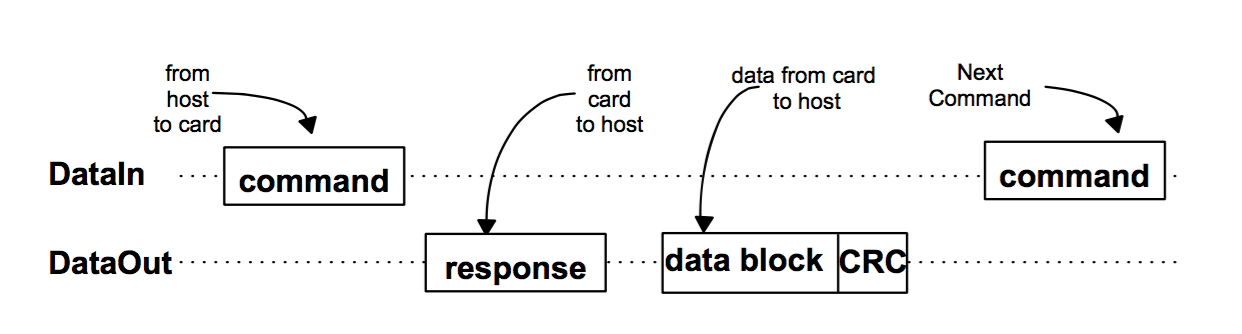
\includegraphics[width=14cm]{chap3/dataread.png}
    \\
    \caption{单块数据读出} \label{fig:dataread}
\end{figure}

一个合法的数据块总会有一个16位的CRC后缀,其由标准CCITT多项式『$x^{16} + x^{12} + x^5 + 1$』生成。
数据块长度的最大值为512字节,无论CSD中定义的「READ\_BL\_LEN」值为多少。
如果部分块访问允许(「READ\_BL\_PARTIAL」等于1),那么块大小可以取1至512字节间的任意值。否则块大小只能是512字节。
至于起始地址可以是任意能够访问的字节地址。

但是对SDHC和SDXC而言,它们只能够支持512字节的块大小。并且起始地址\textbf{必须}和块边界对齐。

当数据检索出错时,SD卡不会传送任何数据。相应地,它会向主机发送一个特定的数据出错令牌(Data Error Token),
图\ref{fig:readerr}显示了在出错时从卡会向主机发送一个出错令牌来取代数据块。

\begin{figure}[!htb]
    \centering
    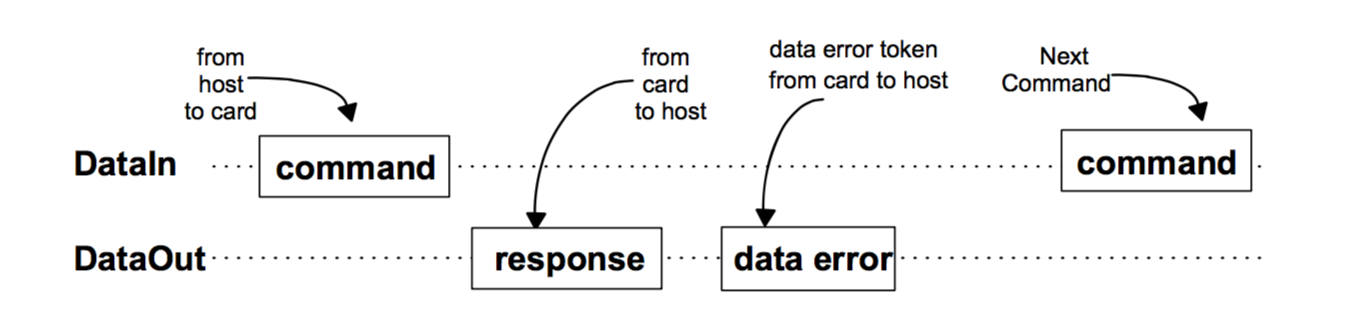
\includegraphics[width=14cm]{chap3/readerr.png}
    \\
    \caption{读操作中数据出错} \label{fig:readerr}
\end{figure}

\subsection{写数据}
\label{sec:datawrite}

SPI模式下支持单块写或多块写(即SD协议中的CMD24或CMD25)。在接收到合法的命令后,
SD卡会发出一个回应,同时开始等待主机传输数据块。图\ref{fig:datawrite}显示了数据块的接受过程。
至于CRC后缀、传输的数据块大小限制和起始地址要求都和读数据(参见章节\ref{sec:dataread})一样,这里不在赘述。

\begin{figure}[!htb]
    \centering
    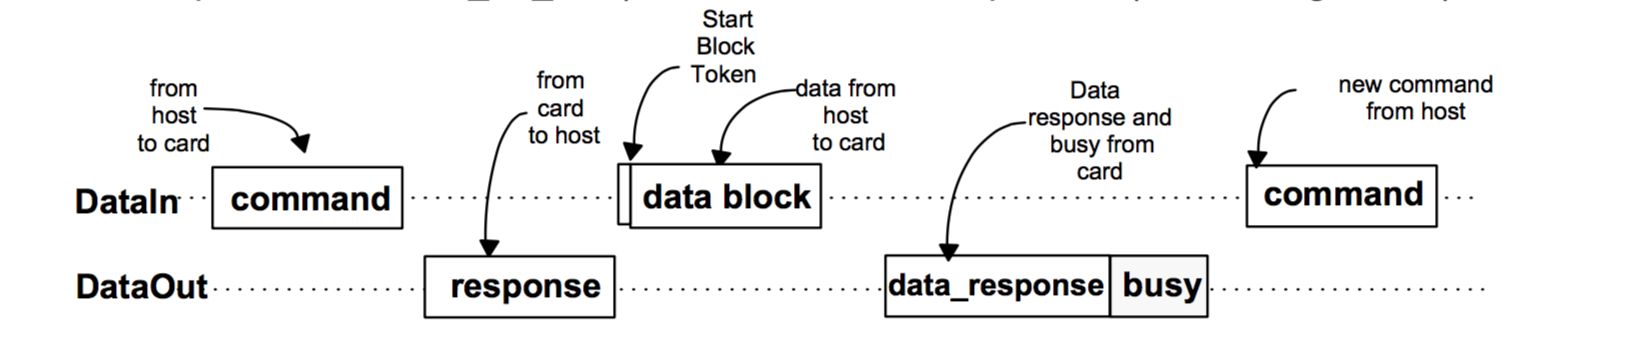
\includegraphics[width=14cm]{chap3/datawrite.png}
    \\
    \caption{单块数据写入} \label{fig:datawrite}
\end{figure}

注意到图\ref{fig:datawrite}中数据块有一个一字节长的前缀:数据起始令牌(Start Block Token)。
在一个数据块写入后,从卡发出一个数据回应令牌(Data Response Token),如果数据块接受正确,
SD卡将开始运行程序写物理数据,同时不停向主机发送忙信号(BUSY),具体表现为MISO引脚被拉低。
一旦程序结束,主机应该通过命令「SEND\_STATUS」(CMD13)检查运行结果,一些错误(比如地址越界)只有在这期间才会被检查到。

当SD卡处于「忙」状态时,重置CS信号并不会中止其进程,此时SD卡将释放MISO(DO数据线)并继续运行程序。
如果卡在程序未完成时被重新选中(通过CS片选),它的DO数据线将被强行拉低并且拒绝一切命令。
特别地,复位命令(CMD0)会终结一切待运行或正在运行的程序进程,同时这将破坏SD卡上的数据格式,
主机有责任避免这种事件的发生。

读写数据块时必须按块按扇区读写,不能够跨扇区地址读写。具体的读写函数很简单,这里就不赘述了。
读写步骤严格按照第\ref{sec:dataread}和\ref{sec:datawrite}节的内容即可,要注意的是,写数据时,在发送写数据令牌(0xFE)之前需要等待至少8个时钟,图\ref{fig:ws}描述了这一过程,当然,
通常的做法是发送若干dummy字节。
\begin{figure}[!htb]
    \centering
    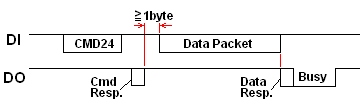
\includegraphics{chap4/ws.png}
    \\
    \caption{写数据块的具体过程}\label{fig:ws}
\end{figure}

整个文件接口的实现过程都必须和底层的硬件相契合,对于不同的硬件或者不同的环境,都要求做出相应的调整。
本工程实现过程中用到了以C8051F020为MCU的单片机,同时用到了一个SD卡槽,该卡槽是11脚卡槽,
比正常的9脚SD卡多了两个保护引脚,其中一个保护引脚是卡插入检测位「CD」,
然而该引脚并没有接在SD卡的「CD/DAT3」引脚上。对于11脚的卡槽,「DAT3」脚与SD卡的「CD/DAT3」相连接。
还有一点需要注意,在C8051F02x系列的芯片的硬件SPI中,NSS位是输入信号,只做从机片选,不能用做CS输出片选。
但在有些型号的芯片的硬件SPI中,NSS即可以做输出又可做输入。


\section{SPI模式下传输的数据分组}
\label{sec:spipack}

\subsection{命令令牌}
\label{sec:cmdtoken}

所有SD卡的命令\footnote{无论SPI模式还是SD模式}都是六个字节,并且传输时总是先传输最左的最高位。
所有命令都被CRC校验位保护\footnote{SPI模式下命令的CRC校验情况见章节\ref{sec:datatrans}}。
命令的具体格式和参数见表\ref{tab:cmdfmt}。
\begin{table}[!htb]
    \centering
    \caption{命令格式} \label{tab:cmdfmt}
    \begin{tabular}{l*{6}{c}}
        \toprule
        位置 & 47 & 46 & [45:40] & [39:8] & [7:1] & 0 \\ \midrule
        长度 & 1 & 1 & 6 & 32 & 7 & 1 \\ \midrule
        值 & `0' & `1' & x & x & x & `1' \\ \midrule
        描述 & 起始位 & 传输位 & 命令号 & 参数 & 7位CRC校验 & 结束位 \\
        \bottomrule
    \end{tabular}
\end{table}

接下来的表\ref{tab:cmddetail}将具体描述各个命令的细节和参数(在SPI模式下的),命令的响应将在第\ref{sec:resp}节说明。
如果一个命令不需要参数,那么其中间的4个字节将被置零。命令的首字节的后六位是命令号,由命令序号的二进制码组成。
例如,「000000」是CMD0的命令号,「100111」是CMD39的命令号。
SD卡将忽略参数中的填充值(STUFF BITS)和保留值(RESERVED BITS)。
\begin{longtable}[!htb]{cp{3cm}ccp{3cm}}
    \caption{命令及参数细节} \label{tab:cmddetail} \\
        \toprule
        命令号 & 参数 & 应答 & 缩略语 & 命令描述 \\ \midrule
        CMD0 & [31:0]填充值 & R1 & GO\_IDLE\_STATE & 复位SD卡。 \\ \midrule
        CMD8\footnote{CMD8是在Version 2.0之后才添加的。} & [31:12]保留位;[11:8]支持的电压(VHS);[7:0]检查 &
            R7 & SEND\_IF\_COND & 发送包含主机支持的电压参数在内的SD卡接口信息,同时询问SD卡电压范围是否合适。
            保留位需置零。\\ \midrule
        CMD17 & [31:0]数据地址\footnote{SDSC卡(CCS=0)使用字节地址,SDHC、SDXC卡(CCS=1)使用块地址(512字节)。}
                & R1 & READ\_SINGLE\_BLOCK & 读一个数据块。 \\ \midrule
        CMD24 & [31:0]数据地址
                 & R1 & WRITE\_BLOCK & 写一个数据块。 \\ \midrule
        CMD32 & [31:0]数据地址
                 & R1 & ERASE\_WR\_BLK\_START\_ADDR & 擦除扇区的首地址。\\ \midrule
        CMD33 & [31:0]数据地址
                 & R1 & ERASE\_WR\_BLK\_END\_ADDR & 擦除扇区的结束地址。 \\ \midrule
        CMD38 & [31:0]填充值 & R1b & ERASE & 擦除之前选定的所有数据块。 \\ \midrule
        CMD55 & [31:0]填充值 & R1 & APP\_CMD & 告诉从卡下一个命令是具体应用命令而不是标准命令。\\ \midrule
        CMD58 & [31:0]填充值 & R3 & READ\_OCR & 读SD卡的OCR寄存器。CCS位被分配在OCR[30]。\\ \midrule
        ACMD41 & [31]保留位;[30]HCS;[29:0]保留位 & R1 & SD\_SEND\_OP\_COND & 
            发送主机的容量支持信息同时激活初始化进程。保留位置零。\\
        \bottomrule
\end{longtable}
表\ref{tab:cmd8}则详细说明了CMD8在SPI模式下SD卡的具体响应。
\begin{table}[!htb]
    \centering
    \caption{SD卡对CMD8具体响应} \label{tab:cmd8}
    \begin{threeparttable}
    \begin{tabular}{*{9}{c}}
        \toprule
        \multicolumn{5}{c}{命令参数检查} & \multicolumn{4}{c}{卡的应答\tnote{1}}\\
        \cmidrule(r){1-5} \cmidrule(r){6-9}
        命令号 & 保留位 & VHS & 模式 & CRC & R1 & 保留位 & VCA & 模式 \\ \midrule
        =8 & 忽略 & 忽略 & 忽略 & 错误 & 0x09 & \multicolumn{3}{c}{(只返回R1)} \\ \midrule
        $\neq$8 & 忽略 & 忽略 & 忽略 & 忽略 & \multicolumn{4}{c}{取决于命令号}\\ \midrule
        =8 & 忽略 & 未匹配\tnote{2} & 忽略 & 正确 & 0x01 & 0 & 0 & 回应 \\ \midrule
        =8 & 忽略 & 匹配\tnote{2} & 忽略 & 正确 & 0x01 & 0 & 回应 & 回应 \\
        \bottomrule
    \end{tabular}
    \begin{tablenotes}
          \item [1] 此处的应答指的是SD卡实际返回的应答(不包含传输应答时发生的错误)。
          \item [2] 「匹配」指\textbf{同时}满足条件a)和b),「未匹配」是其他情形:
           a)VHS中只有一位被置「1」;b)从卡符合主机电压参数。
    \end{tablenotes}
    \end{threeparttable}
\end{table}


\subsection{应答令牌}
\label{sec:resp}

在SD卡中存在多种形式的应答令牌,SPI模式和SD模式都是最先传送最高位(MSB)。
SPI中不仅有单字节的应带(如R1),还有多字节的应答(如R3)。但是,当命令出错或者CRC校验出错时,
SD卡仅会输出一个字节(形式和R1相同),此时主机只需度一个字节的响应即可。
限于篇幅,本章进介绍几个常用的应答令牌,其他的应答可以参阅相关资料。

\subsubsection{R1格式}
\label{sec:r1}

此应答令牌会在SD卡接受到每一个命令后发送给主机,可以直接作为应答令牌,也可以作为应答令牌的一部分(如R3)。
但是,命令「SEND\_STATUS」除外\footnote{此命令的应答令牌为R2,和R1形式不同,不相互包含}。
R1令牌长度一个字节,且最高位(MSB)永远置零,其他位均是错误提示,出错时置一。令牌结构见图\ref{fig:r1},
每一位的具体信息为:
\begin{itemize}
    \item 空闲状态: SD卡处于空闲状态,正在初始化进程。
    \item 擦除重置: 擦除序列在执行前被清空,因为收到了不在其序列中的命令。
    \item 非法命令: 检测到不合法命令。
    \item CRC出错:  最后一个命令的CRC校验出错。
    \item 擦除序列出错:擦除序列中检测到错误。
    \item 地址错误:命令中出现未与数据块边界对齐的地址。
    \item 参数错误: 命令参数超出SD卡允许的范围。
\end{itemize}

\begin{figure}[!htb]
    \centering
    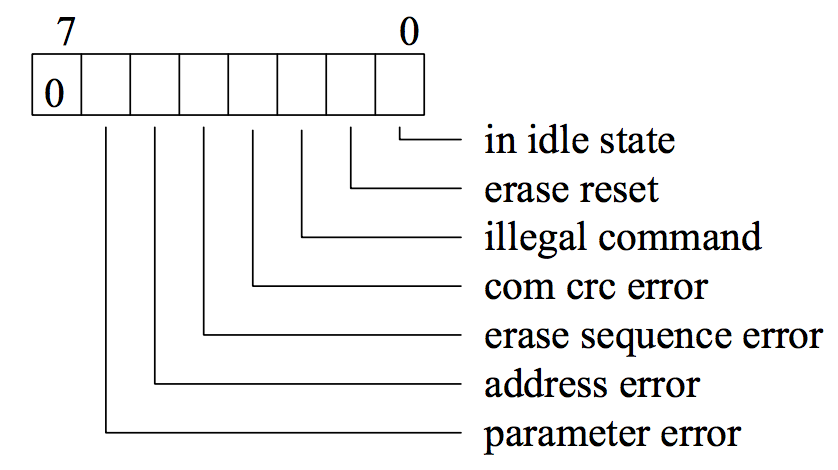
\includegraphics[height=4cm]{chap3/r1.png}
    \\
    \caption{应答令牌R1的格式}\label{fig:r1}
\end{figure}

\subsubsection{R3格式}
\label{sec:r3}

当SD卡收到命令「READ\_OCR」时将会发送此应答令牌。该令牌长度5个字节(见图\ref{fig:r3}),且其最高字节(MSB)与R1相同,
之后的四个字节由OCR寄存器的内容组成。

\begin{figure}[!htb]
    \centering
    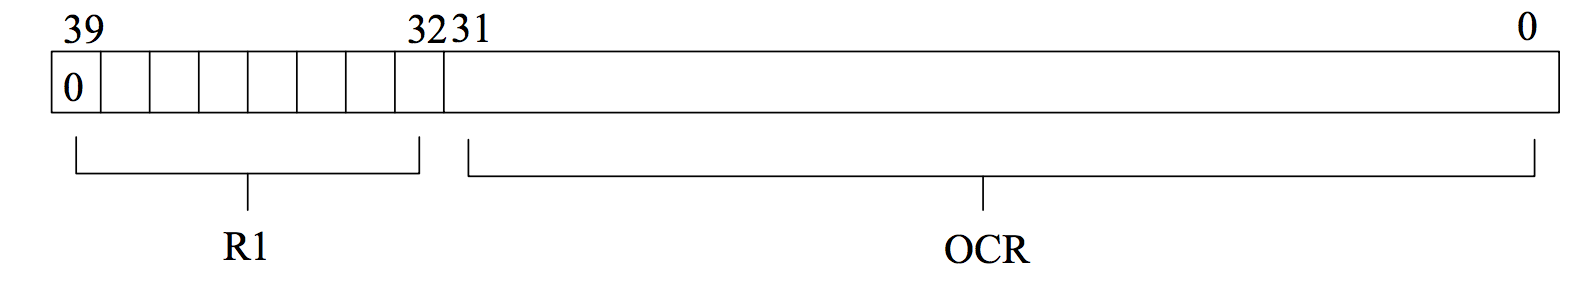
\includegraphics[width=17cm]{chap3/r3.png}
    \\
    \caption{应答令牌R3的格式}\label{fig:r3}
\end{figure}

\subsubsection{R7格式}
\label{sec:r7}

当SD卡收到命令「SEND\_IF\_COND」(CMD8)时会发送此应答令牌。该令牌长度5个字节(见图\ref{fig:r7})。
其首字节(MSB)和R1结构相同,剩下的四个字节包含了SD卡的工作电压信息、命令版本、对检查模式的回应等特殊信息。

\begin{figure}[!htb]
    \centering
    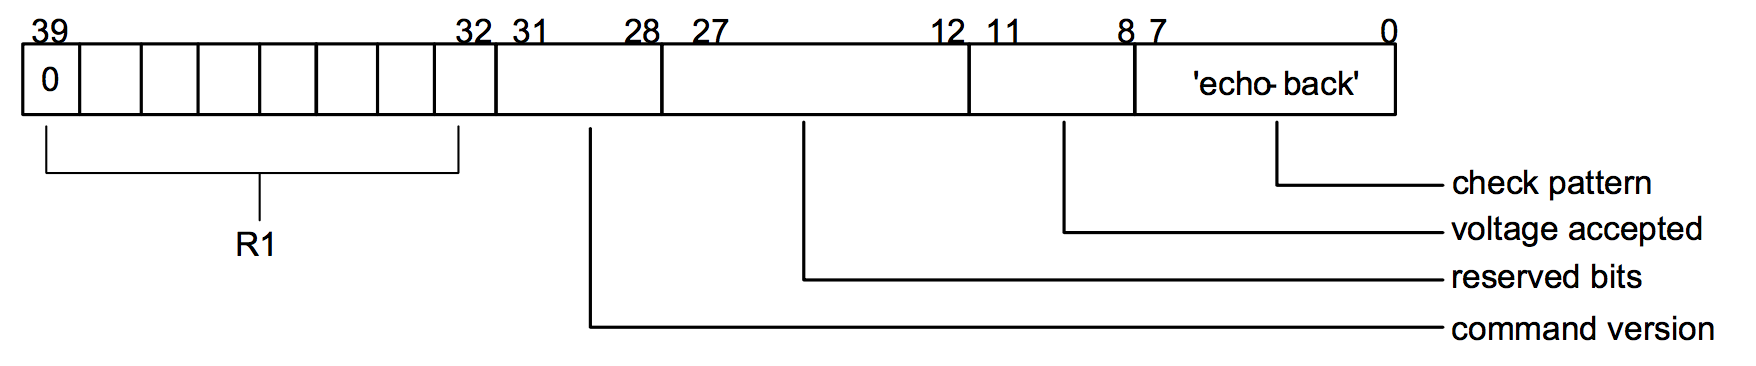
\includegraphics[width=17cm]{chap3/r7.png}
    \\
    \caption{应答令牌R7的格式}\label{fig:r7}
\end{figure}


\subsection{控制令牌}
\label{sec:ctrltoken}

数据块的传输是由以下这些令牌所控制。

\subsubsection{数据应答令牌}
\label{sec:dataresp}
每当一个数据块写入SD卡时,SD卡将回应一个单字节的数据应答令牌以表示收到。
它的高三位可以是任意值(b7-b5),第四位(b4)和第零位(b0)必须分别为「0」和「1」。
中间三位(b3-b1)的取值如下:
\begin{itemize}
    \item 「010」数据已接收
    \item 「101」拒绝接收因为CRC错误
    \item 「110」拒绝接收因为写入出错
\end{itemize}

\subsubsection{数据块起始令牌}
\label{sec:stbltran}

数据块的传送与接收将通过数据块起始令牌完成,所有数据都将从最高字节(MSB)开始传送。
\begin{itemize}
    \item 第一字节:数据块起始令牌「0xFE」
    \item 中间字节\footnote{具体情况视数据块长度而定}(2-513):数据信息
    \item 最后两个字节:16位的CRC校验
\end{itemize}

\subsubsection{数据出错令牌}
\label{sec:dataerr}

如果读操作出错\footnote{可以参见第\ref{sec:dataread}节},SD卡将返回一个数据出错令牌来取代原本应该读出的数据。
该令牌长一个字节,高四位(b7-b4)全部为零,第四位(b3-b0)分别为:出界、CRC出错、
CC错\footnote{Internal Card Controller Error,内部卡控制器出错}和出错\footnote{通常错误或未知错误}。

\section{本章小结}
\label{sec:sum3}
本章不仅简述了SD卡物理结构,更是详尽描述了SD卡在SPI模式下的具体工作方式,作为底层子模块,
必须为上层模块提供可用的接口函数,同时与硬件紧密结合,做好上层软件与底层硬件的通信工作。
本章的重点在于SD卡上电复位后进入SPI模式的一系列命令序列和判断过程,因为初始化完成后SD卡的读写操作都比较容易实现,
然而,初始化流程实际建立在正确地命令与应答基础上。因此,本章对SPI模式下能用到的命令和
应答令牌都做了比较详细的说明。
